% Options for packages loaded elsewhere
\PassOptionsToPackage{unicode}{hyperref}
\PassOptionsToPackage{hyphens}{url}
%
\documentclass[
  american,
  man]{apa7}
\usepackage{amsmath,amssymb}
\usepackage{lmodern}
\usepackage{ifxetex,ifluatex}
\ifnum 0\ifxetex 1\fi\ifluatex 1\fi=0 % if pdftex
  \usepackage[T1]{fontenc}
  \usepackage[utf8]{inputenc}
  \usepackage{textcomp} % provide euro and other symbols
\else % if luatex or xetex
  \usepackage{unicode-math}
  \defaultfontfeatures{Scale=MatchLowercase}
  \defaultfontfeatures[\rmfamily]{Ligatures=TeX,Scale=1}
\fi
% Use upquote if available, for straight quotes in verbatim environments
\IfFileExists{upquote.sty}{\usepackage{upquote}}{}
\IfFileExists{microtype.sty}{% use microtype if available
  \usepackage[]{microtype}
  \UseMicrotypeSet[protrusion]{basicmath} % disable protrusion for tt fonts
}{}
\makeatletter
\@ifundefined{KOMAClassName}{% if non-KOMA class
  \IfFileExists{parskip.sty}{%
    \usepackage{parskip}
  }{% else
    \setlength{\parindent}{0pt}
    \setlength{\parskip}{6pt plus 2pt minus 1pt}}
}{% if KOMA class
  \KOMAoptions{parskip=half}}
\makeatother
\usepackage{xcolor}
\IfFileExists{xurl.sty}{\usepackage{xurl}}{} % add URL line breaks if available
\IfFileExists{bookmark.sty}{\usepackage{bookmark}}{\usepackage{hyperref}}
\hypersetup{
  pdftitle={Integration of Migrants: Annotated Analysis},
  pdfauthor={Jannis Kreienkamp1,2, Kai Epstude1,2, Laura F. Bringmann1,2, \& Peter de Jonge1,2},
  pdflang={en-US},
  pdfkeywords={Acculturation, Integration, Systematic Review},
  hidelinks,
  pdfcreator={LaTeX via pandoc}}
\urlstyle{same} % disable monospaced font for URLs
\usepackage{longtable,booktabs,array}
\usepackage{calc} % for calculating minipage widths
% Correct order of tables after \paragraph or \subparagraph
\usepackage{etoolbox}
\makeatletter
\patchcmd\longtable{\par}{\if@noskipsec\mbox{}\fi\par}{}{}
\makeatother
% Allow footnotes in longtable head/foot
\IfFileExists{footnotehyper.sty}{\usepackage{footnotehyper}}{\usepackage{footnote}}
\makesavenoteenv{longtable}
\usepackage{graphicx}
\makeatletter
\def\maxwidth{\ifdim\Gin@nat@width>\linewidth\linewidth\else\Gin@nat@width\fi}
\def\maxheight{\ifdim\Gin@nat@height>\textheight\textheight\else\Gin@nat@height\fi}
\makeatother
% Scale images if necessary, so that they will not overflow the page
% margins by default, and it is still possible to overwrite the defaults
% using explicit options in \includegraphics[width, height, ...]{}
\setkeys{Gin}{width=\maxwidth,height=\maxheight,keepaspectratio}
% Set default figure placement to htbp
\makeatletter
\def\fps@figure{htbp}
\makeatother
\setlength{\emergencystretch}{3em} % prevent overfull lines
\providecommand{\tightlist}{%
  \setlength{\itemsep}{0pt}\setlength{\parskip}{0pt}}
\setcounter{secnumdepth}{-\maxdimen} % remove section numbering
% Make \paragraph and \subparagraph free-standing
\ifx\paragraph\undefined\else
  \let\oldparagraph\paragraph
  \renewcommand{\paragraph}[1]{\oldparagraph{#1}\mbox{}}
\fi
\ifx\subparagraph\undefined\else
  \let\oldsubparagraph\subparagraph
  \renewcommand{\subparagraph}[1]{\oldsubparagraph{#1}\mbox{}}
\fi
% Manuscript styling
\usepackage{upgreek}
\captionsetup{font=singlespacing,justification=justified}

% Table formatting
\usepackage{longtable}
\usepackage{lscape}
% \usepackage[counterclockwise]{rotating}   % Landscape page setup for large tables
\usepackage{multirow}		% Table styling
\usepackage{tabularx}		% Control Column width
\usepackage[flushleft]{threeparttable}	% Allows for three part tables with a specified notes section
\usepackage{threeparttablex}            % Lets threeparttable work with longtable

% Create new environments so endfloat can handle them
% \newenvironment{ltable}
%   {\begin{landscape}\begin{center}\begin{threeparttable}}
%   {\end{threeparttable}\end{center}\end{landscape}}
\newenvironment{lltable}{\begin{landscape}\begin{center}\begin{ThreePartTable}}{\end{ThreePartTable}\end{center}\end{landscape}}

% Enables adjusting longtable caption width to table width
% Solution found at http://golatex.de/longtable-mit-caption-so-breit-wie-die-tabelle-t15767.html
\makeatletter
\newcommand\LastLTentrywidth{1em}
\newlength\longtablewidth
\setlength{\longtablewidth}{1in}
\newcommand{\getlongtablewidth}{\begingroup \ifcsname LT@\roman{LT@tables}\endcsname \global\longtablewidth=0pt \renewcommand{\LT@entry}[2]{\global\advance\longtablewidth by ##2\relax\gdef\LastLTentrywidth{##2}}\@nameuse{LT@\roman{LT@tables}} \fi \endgroup}

% \setlength{\parindent}{0.5in}
% \setlength{\parskip}{0pt plus 0pt minus 0pt}

% Overwrite redefinition of paragraph and subparagraph by the default LaTeX template
% See https://github.com/crsh/papaja/issues/292
\makeatletter
\renewcommand{\paragraph}{\@startsection{paragraph}{4}{\parindent}%
  {0\baselineskip \@plus 0.2ex \@minus 0.2ex}%
  {-1em}%
  {\normalfont\normalsize\bfseries\itshape\typesectitle}}

\renewcommand{\subparagraph}[1]{\@startsection{subparagraph}{5}{1em}%
  {0\baselineskip \@plus 0.2ex \@minus 0.2ex}%
  {-\z@\relax}%
  {\normalfont\normalsize\itshape\hspace{\parindent}{#1}\textit{\addperi}}{\relax}}
\makeatother

% \usepackage{etoolbox}
\makeatletter
\patchcmd{\HyOrg@maketitle}
  {\section{\normalfont\normalsize\abstractname}}
  {\section*{\normalfont\normalsize\abstractname}}
  {}{\typeout{Failed to patch abstract.}}
\patchcmd{\HyOrg@maketitle}
  {\section{\protect\normalfont{\@title}}}
  {\section*{\protect\normalfont{\@title}}}
  {}{\typeout{Failed to patch title.}}
\makeatother
\shorttitle{integration of migrants -- analysis}
\keywords{Acculturation, Integration, Systematic Review\newline\indent Word count: 3}
\DeclareDelayedFloatFlavor{ThreePartTable}{table}
\DeclareDelayedFloatFlavor{lltable}{table}
\DeclareDelayedFloatFlavor*{longtable}{table}
\makeatletter
\renewcommand{\efloat@iwrite}[1]{\immediate\expandafter\protected@write\csname efloat@post#1\endcsname{}}
\makeatother
\usepackage{csquotes}
\ifxetex
  % Load polyglossia as late as possible: uses bidi with RTL langages (e.g. Hebrew, Arabic)
  \usepackage{polyglossia}
  \setmainlanguage[variant=american]{english}
\else
  \usepackage[main=american]{babel}
% get rid of language-specific shorthands (see #6817):
\let\LanguageShortHands\languageshorthands
\def\languageshorthands#1{}
\fi
\ifluatex
  \usepackage{selnolig}  % disable illegal ligatures
\fi
\newlength{\cslhangindent}
\setlength{\cslhangindent}{1.5em}
\newlength{\csllabelwidth}
\setlength{\csllabelwidth}{3em}
\newenvironment{CSLReferences}[2] % #1 hanging-ident, #2 entry spacing
 {% don't indent paragraphs
  \setlength{\parindent}{0pt}
  % turn on hanging indent if param 1 is 1
  \ifodd #1 \everypar{\setlength{\hangindent}{\cslhangindent}}\ignorespaces\fi
  % set entry spacing
  \ifnum #2 > 0
  \setlength{\parskip}{#2\baselineskip}
  \fi
 }%
 {}
\usepackage{calc}
\newcommand{\CSLBlock}[1]{#1\hfill\break}
\newcommand{\CSLLeftMargin}[1]{\parbox[t]{\csllabelwidth}{#1}}
\newcommand{\CSLRightInline}[1]{\parbox[t]{\linewidth - \csllabelwidth}{#1}\break}
\newcommand{\CSLIndent}[1]{\hspace{\cslhangindent}#1}

\title{Integration of Migrants: Annotated Analysis}
\author{Jannis Kreienkamp\textsuperscript{1,2}, Kai Epstude\textsuperscript{1,2}, Laura F. Bringmann\textsuperscript{1,2}, \& Peter de Jonge\textsuperscript{1,2}}
\date{}


\authornote{

\addORCIDlink{* Jannis Kreienkamp}{0000-0002-1831-5604}

We have no known conflict of interest to declare.

Correspondence concerning this article should be addressed to Jannis Kreienkamp, Grote Kruisstraat 2/1, 9712 TS Groningen, The Netherlands. E-mail: \href{mailto:j.kreienkamp@rug.nl}{\nolinkurl{j.kreienkamp@rug.nl}}

}

\affiliation{\vspace{0.5cm}\textsuperscript{1} University of Groningen; Department of Psychology\\\textsuperscript{2} Author order still to be decided (sorted alphabetically by first name)}

\abstract{
Abstract goes here.
}



\begin{document}
\maketitle

\hypertarget{data-preparation}{%
\section{Data Preparation}\label{data-preparation}}

\hypertarget{import-data}{%
\subsection{Import Data}\label{import-data}}

In a first step we import the raw data of the review from the shared coding \href{https://docs.google.com/spreadsheets/d/1j3j7q15lhNqPxp3qGnRtc2zuaE7plxWYR7tWKltkdU8/edit?usp=sharing}{Google Sheet}. We, primarily, import the database of the scale validations and the review of the empirical papers. Beyond that we also import the separate lists of codes used.

\hypertarget{prepare-data-frames}{%
\subsection{Prepare Data Frames}\label{prepare-data-frames}}

We then go on to clean the data sets in order to use them in later analyses and keep track of exclusion filters.

\hypertarget{analysis}{%
\section{Analysis}\label{analysis}}

\hypertarget{scale-validations}{%
\subsection{Scale Validations}\label{scale-validations}}

The first data set we assess is a database of scale validations. We bring together the scales suggested in previous reviews as well as validation studies we identified in our own review. Throughout our literature review we found five major reviews that reviewed the measurement of acculturation (Celenk \& Van de Vijver, 2011; Maestas, 2000; Matsudaira, 2006; Wallace et al., 2010; Zane \& Mak, 2004).

\hypertarget{exclusions}{%
\subsubsection{Exclusions}\label{exclusions}}

Taken together these five reviews collected a total of 197 scales, of which 75 were duplicates. From our own review we added 25 additional validation studies. After removing duplicates this meant that we considered a total of 122 unique scales for our coding. Of these scales we ultimately had to exclude 41, because they were either not accessible or did not fit the the topic of our review (see Table \ref{tab:ScalesExclusion}).

\begin{table}

\caption{\label{tab:ScalesExclusion}Reasons for Exclusion}
\begin{tabular}[t]{lc}
\toprule
Exclusion Reason & Frequency\\
\midrule
not migration & 14\\
items not included & 8\\
search pending & 5\\
not accessible & 4\\
not found & 3\\
\addlinespace
not acculturation & 2\\
majority focussed & 1\\
not found probably the same as Tsai et al. 2000 & 1\\
only language (no scale) & 1\\
same as S-029 & 1\\
\addlinespace
uses other scale & 1\\
\bottomrule
\end{tabular}
\end{table}

The remaining 87 scales are listed in the HTML version as well as on OSF (table too large for PDF).

\hypertarget{interest-over-time}{%
\subsubsection{Interest over time}\label{interest-over-time}}

Of the scale we included we also plotted the publication years of the scale validations in order to gain an understanding of the interest in scale development over time.

\begin{figure}
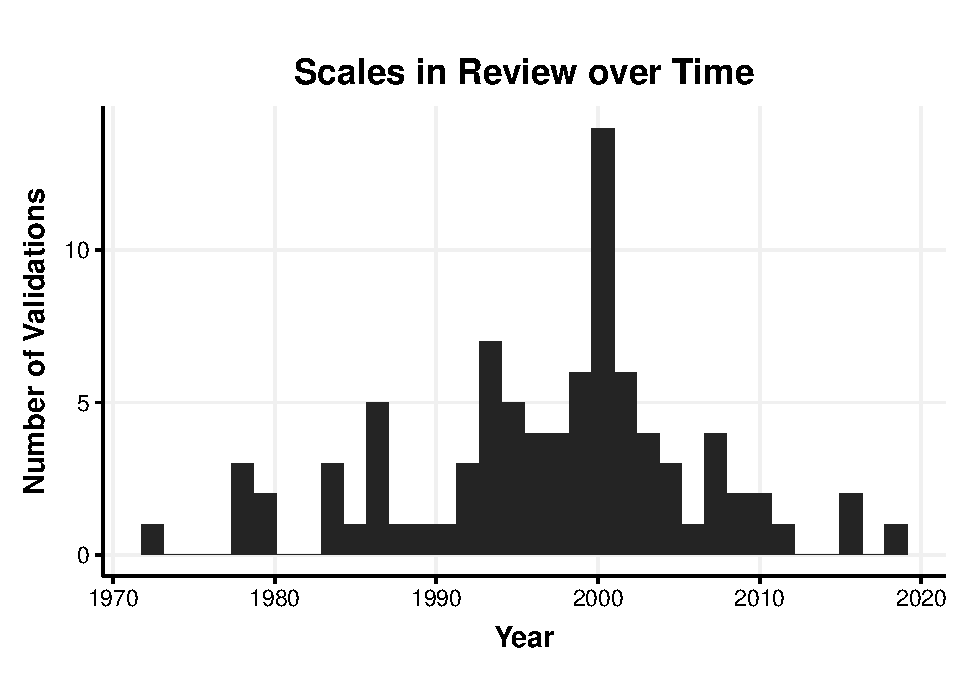
\includegraphics[width=\textwidth]{Figures/HistTime-1} \caption{Histogram of Scale Validations over Time.}\label{fig:HistTime}
\end{figure}

\hypertarget{sample}{%
\subsubsection{Sample}\label{sample}}

The study sample a scale is validated in can be fairly important if one plans to use a scale for a context-specific phenomenon such as a cultural adaptation of two specific cultures. We, therefore, coded the type of sample the original authors used in their validation studies (see Figure \ref{fig:SampleFreq}).

\begin{figure}
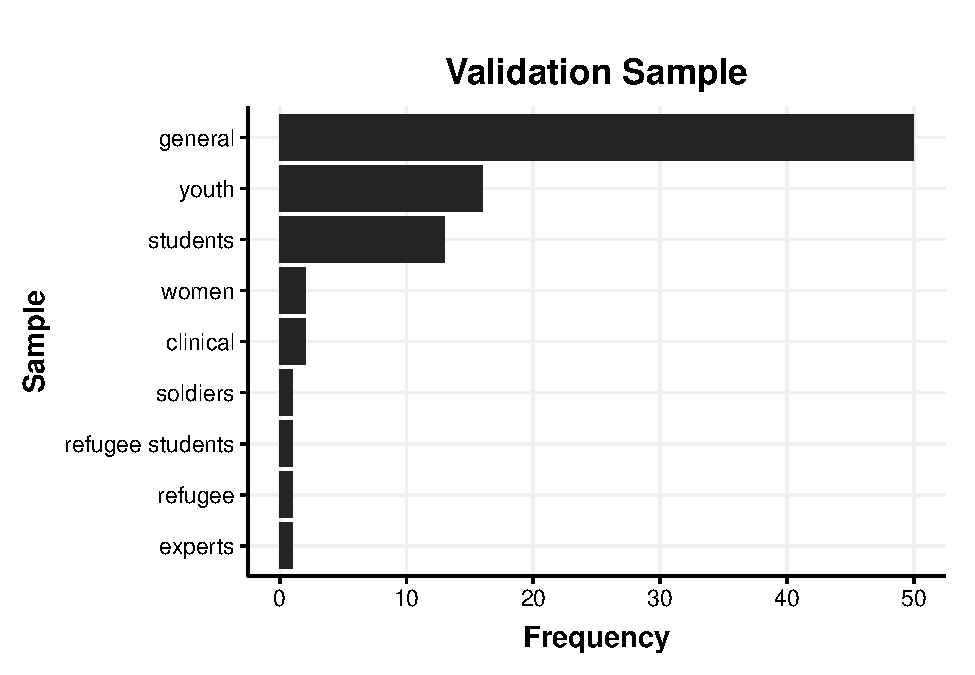
\includegraphics[width=\textwidth]{Figures/SampleFreq-1} \caption{Bar graph of the study samples used in the original validation studies.}\label{fig:SampleFreq}
\end{figure}

\hypertarget{dimensions}{%
\subsubsection{Dimensions}\label{dimensions}}

One major focus of our coding efforts was put on identifying the phenomenological dimensions that were assessed by each individual scale. Based the ABCD framework of human experiences, we independently distinguished between emotional (affect), behavioral, cognitive, and need-based measurements of of acculturation. Examples of concepts that fell into the individual dimensions are shown in Table \ref{tab:Dimensions}:\\

\begin{longtable}[]{@{}
  >{\raggedright\arraybackslash}p{(\columnwidth - 4\tabcolsep) * \real{0.08}}
  >{\raggedright\arraybackslash}p{(\columnwidth - 4\tabcolsep) * \real{0.52}}
  >{\raggedright\arraybackslash}p{(\columnwidth - 4\tabcolsep) * \real{0.39}}@{}}
\caption{\label{tab:Dimensions} Examples for Dimensions of Acculturation Measurements.}\tabularnewline
\toprule
Dimension & Concept & Wording \\ \addlinespace
\midrule
\endfirsthead
\toprule
Dimension & Concept & Wording \\ \addlinespace
\midrule
\endhead
Affect & belonging, loneliness, satisfaction & ``I feel \ldots{},'' \\ \addlinespace
Behavior & language learning, media consumption, voting & ``I do \ldots{},'' ``I speak \ldots{},'' ``I meet \ldots{}'' \\ \addlinespace
Cognition & cultural identification, cultural values, attitude towards majority & ``I prefer \ldots{},'' ``I think \ldots{},'' ``I identify as \ldots{}'' \\ \addlinespace
Desire & needs, goals, wants & ``I want \ldots{},'' ``I would like to \ldots{},'' ``I need \ldots{}'' \\ \addlinespace
\bottomrule
\end{longtable}

Note that this also means that we do not include scales that measure aspects of acculturation that do can be measured without consideration of the individual's experiences, such as physical changes, cultural changes, or societal changes.

Figure \ref{fig:ABCDFreq} shows how often each of the dimensions was coded.

\begin{figure}
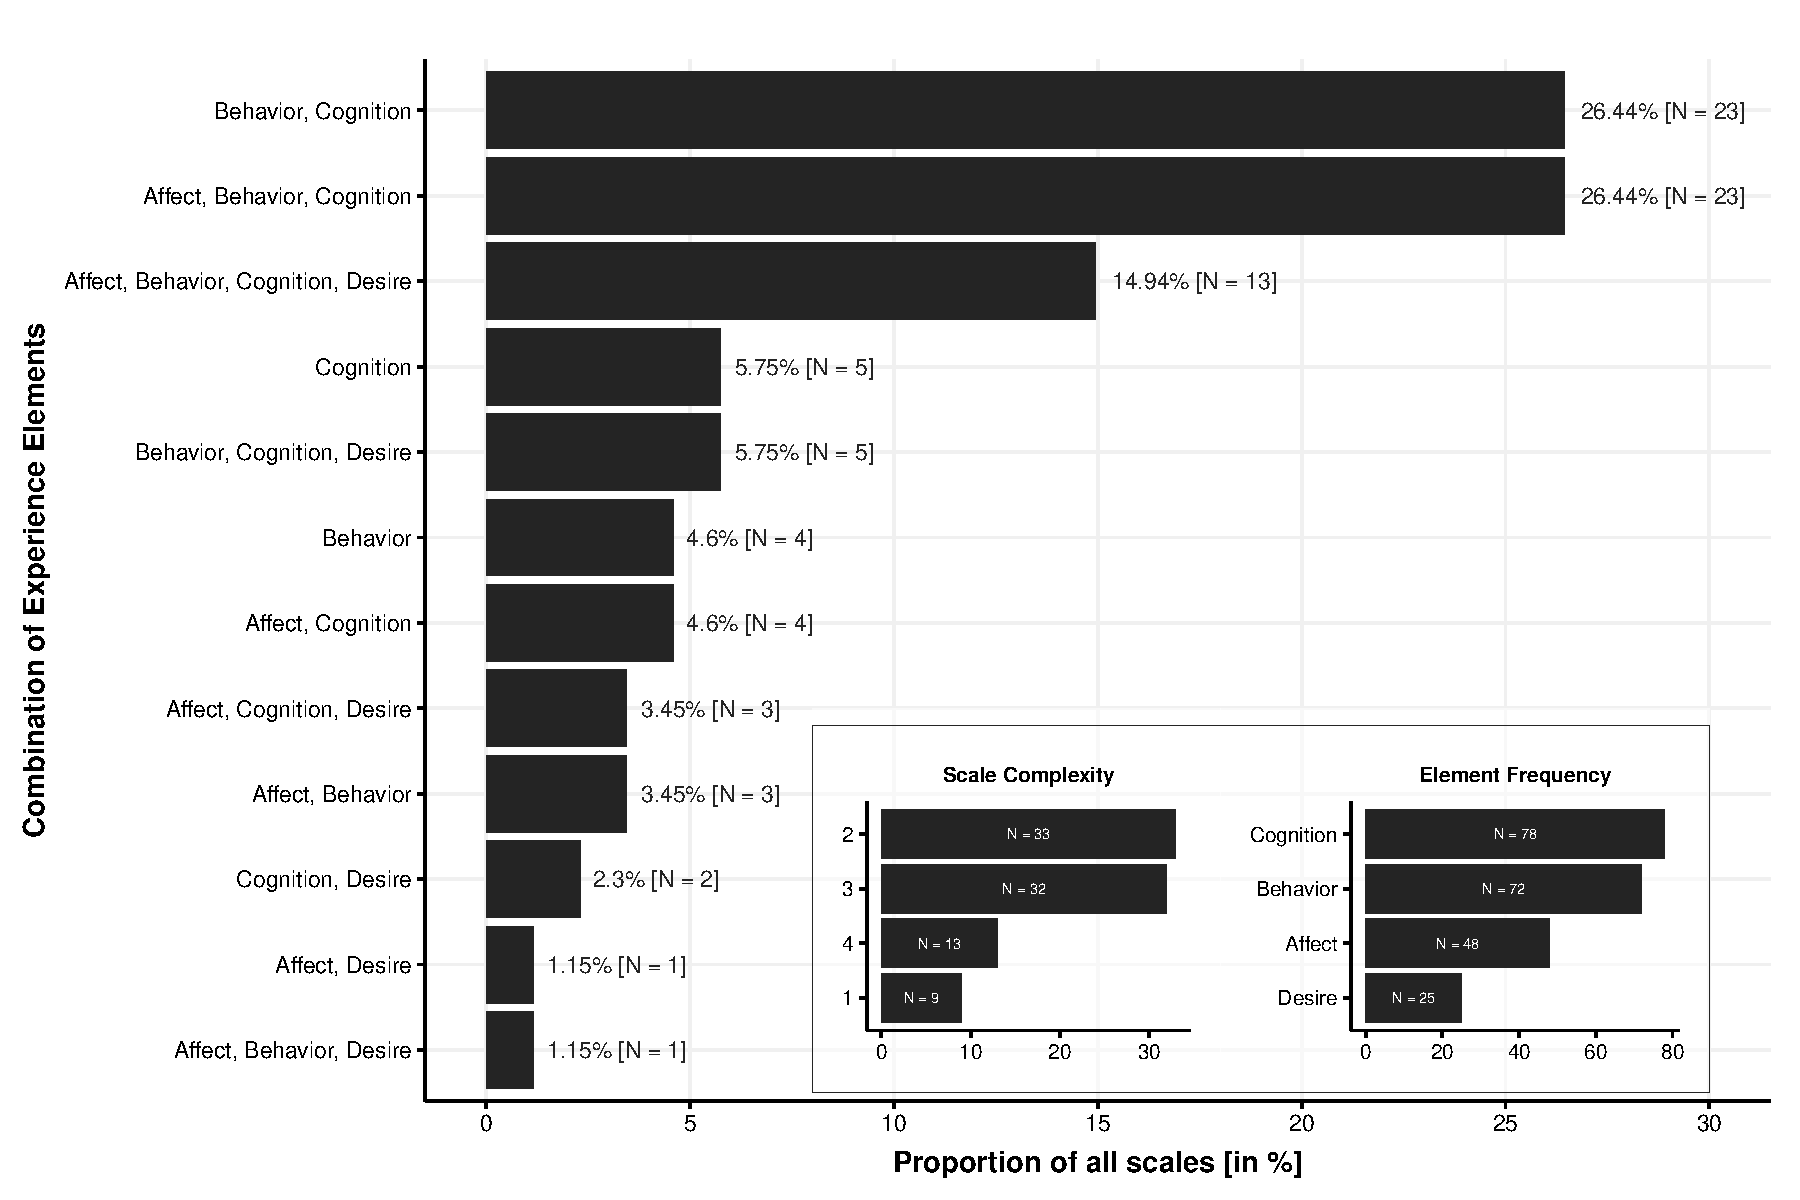
\includegraphics[width=\textwidth]{Figures/ABCDFreq-1} \caption{Bar graph of the counts for each of the dimensions.}\label{fig:ABCDFreq}
\end{figure}

We also plot how often each of the dimensions were measured together. A bar graph of the compound frequencies is shown Figure \ref{fig:ABCDCombFreq} and a network graph of frequencies and co-occurrences is shown in Figure \ref{fig:dimensionNetwork}.

\begin{figure}
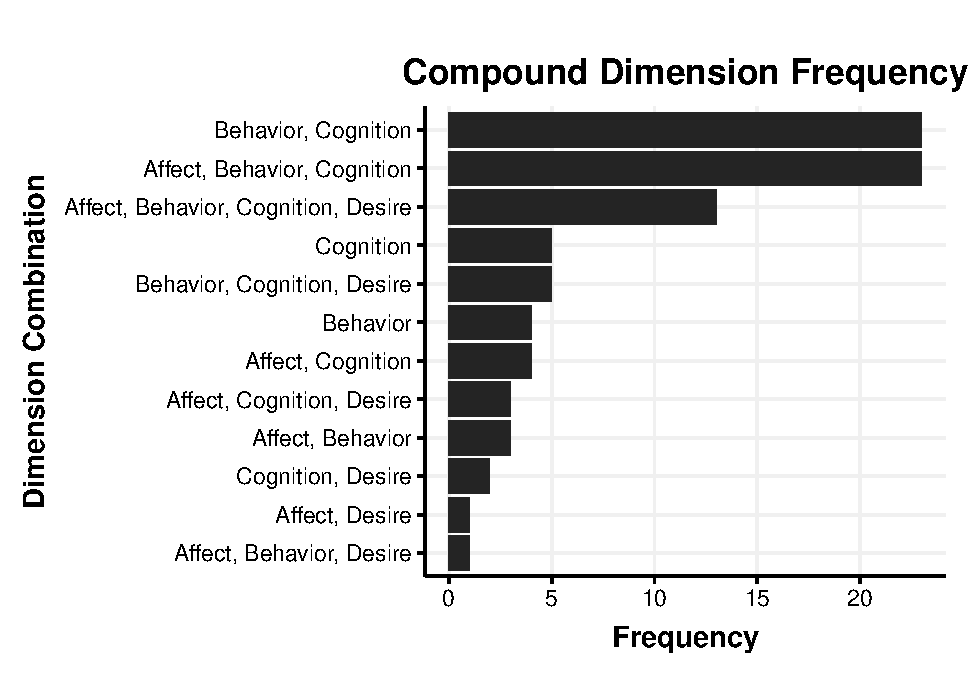
\includegraphics[width=\textwidth]{Figures/ABCDCombFreq-1} \caption{Bar graph of the counts for each of the dimension combinations.}\label{fig:ABCDCombFreq}
\end{figure}

\hypertarget{software-information}{%
\section{Software Information}\label{software-information}}

For our analyses we used R {[}Version 4.0.3; @{]} and the R-packages \emph{\}base} {[}@\}R-base{]}, \emph{bookdown} {[}Version 0.21; Xie (2016){]}, \emph{citr} {[}Version 0.3.2; Aust (2019){]}, \emph{data.table} {[}Version 1.13.0; Dowle and Srinivasan (2020){]}, \emph{dplyr} {[}Version 1.0.2; Wickham et al. (2020){]}, \emph{ellipse} {[}Version 0.4.2; Murdoch and Chow (2020){]}, \emph{forcats} {[}Version 0.5.0; Wickham (2020a){]}, \emph{Formula} {[}Version 1.2.3; Zeileis and Croissant (2010){]}, \emph{GGally} {[}Version 2.0.0; Schloerke et al. (2020){]}, \emph{ggplot2} {[}Version 3.3.2; Wickham (2016){]}, \emph{ggspatial} {[}Version 1.1.4; Dunnington (2020){]}, \emph{ggstatsplot} {[}Version 0.6.5; Patil (2018){]}, \emph{ggthemes} {[}Version 4.2.0; Arnold (2019){]}, \emph{ggwordcloud} {[}Version 0.5.0; Le Pennec and Slowikowski (2019){]}, \emph{gsheet} {[}Version 0.4.5; Conway (2020){]}, \emph{gsubfn} {[}Version 0.7; G. Grothendieck (2018){]}, \emph{haven} {[}Version 2.3.1; Wickham and Miller (2020){]}, \emph{Hmisc} {[}Version 4.4.1; Harrell Jr et al. (2020){]}, \emph{hrbrthemes} {[}Version 0.8.0; Rudis (2020){]}, \emph{ISOcodes} {[}Version 2020.3.16; Buchta and Hornik (2020){]}, \emph{kableExtra} {[}Version 1.2.1.9000; Zhu (2020){]}, \emph{knitr} {[}Version 1.30; Xie (2015){]}, \emph{lattice} {[}Version 0.20.41; Sarkar (2008){]}, \emph{lubridate} {[}Version 1.7.9; Grolemund and Wickham (2011){]}, \emph{mada} {[}Version 0.5.10; Doebler (2020){]}, \emph{matrixStats} {[}Version 0.57.0; Bengtsson (2020){]}, \emph{mvmeta} {[}Version 1.0.3; Gasparrini et al. (2012){]}, \emph{mvtnorm} {[}Version 1.1.1; Genz and Bretz (2009){]}, \emph{naniar} {[}Version 0.6.0; Tierney et al. (2020){]}, \emph{networkD3} {[}Version 0.4; Allaire et al. (2017){]}, \emph{pander} {[}Version 0.6.3; Daróczi and Tsegelskyi (2018){]}, \emph{papaja} {[}Version 0.1.0.9997; Aust and Barth (2020){]}, \emph{plotly} {[}Version 4.9.2.1; Sievert (2020){]}, \emph{proto} {[}Version 1.0.0; Gabor Grothendieck et al. (2016){]}, \emph{psych} {[}Version 2.0.9; Revelle (2020){]}, \emph{RColorBrewer} {[}Version 1.1.2; Neuwirth (2014){]}, \emph{readxl} {[}Version 1.3.1; Wickham and Bryan (2019){]}, \emph{remedy} {[}Version 0.1.1; Fay et al. (2020){]}, \emph{reshape2} {[}Version 1.4.3; Wickham (2007){]}, \emph{rgeos} {[}Version 0.5.5; Bivand and Rundel (2020){]}, \emph{rmarkdown} {[}Version 2.6; Xie et al. (2018); Xie et al. (2020){]}, \emph{rmdfiltr} {[}Version 0.1.3; Aust (2020){]}, \emph{rnaturalearth} {[}Version 0.1.0; South (2017a); South (2017b){]}, \emph{rnaturalearthdata} {[}Version 0.1.0; South (2017b){]}, \emph{RSQLite} {[}Version 2.2.1; Müller et al. (2020){]}, \emph{rworldmap} {[}Version 1.3.6; South (2011){]}, \emph{sp} {[}Version 1.4.4; Dunnington (2020); Patil (2018); Pebesma and Bivand (2005){]}, \emph{sqldf} {[}Version 0.4.11; G. Grothendieck (2017){]}, \emph{stringi} {[}Version 1.5.3; Gagolewski (2020){]}, \emph{stringr} {[}Version 1.4.0; Wickham (2019){]}, \emph{survival} {[}Version 3.1.12; Terry M. Therneau and Patricia M. Grambsch (2000){]}, \emph{tibble} {[}Version 3.0.4; Müller and Wickham (2020){]}, \emph{tidyr} {[}Version 1.1.2; Wickham (2020b){]}, \emph{tinylabels} {[}Version 0.1.0; Barth (2020){]}, \emph{visNetwork} {[}Version 2.0.9; Almende B.V. et al. (2019){]}, and \emph{wordcloud} {[}Version 2.6; Le Pennec and Slowikowski (2019); Fellows (2018){]}.

\newpage

\hypertarget{references}{%
\section{References}\label{references}}

\begingroup
\setlength{\parindent}{-0.5in}
\setlength{\leftskip}{0.5in}

\hypertarget{refs}{}
\begin{CSLReferences}{1}{0}
\leavevmode\hypertarget{ref-R-networkD3}{}%
Allaire, J. J., Gandrud, C., Russell, K., \& Yetman, C. (2017). \emph{networkD3: D3 JavaScript network graphs from r}. \url{https://CRAN.R-project.org/package=networkD3}

\leavevmode\hypertarget{ref-R-visNetwork}{}%
Almende B.V., Thieurmel, B., \& Robert, T. (2019). \emph{visNetwork: Network visualization using 'vis.js' library}. \url{https://CRAN.R-project.org/package=visNetwork}

\leavevmode\hypertarget{ref-R-ggthemes}{}%
Arnold, J. B. (2019). \emph{Ggthemes: Extra themes, scales and geoms for 'ggplot2'}. \url{https://CRAN.R-project.org/package=ggthemes}

\leavevmode\hypertarget{ref-R-citr}{}%
Aust, F. (2019). \emph{Citr: 'RStudio' add-in to insert markdown citations}. \url{https://CRAN.R-project.org/package=citr}

\leavevmode\hypertarget{ref-R-rmdfiltr}{}%
Aust, F. (2020). \emph{Rmdfiltr: 'Lua'-filters for r markdown}. \url{https://CRAN.R-project.org/package=rmdfiltr}

\leavevmode\hypertarget{ref-R-papaja}{}%
Aust, F., \& Barth, M. (2020). \emph{{papaja}: {Prepare} reproducible {APA} journal articles with {R Markdown}}. \url{https://github.com/crsh/papaja}

\leavevmode\hypertarget{ref-R-tinylabels}{}%
Barth, M. (2020). \emph{Tinylabels: Lightweight variable labels}. \url{https://CRAN.R-project.org/package=tinylabels}

\leavevmode\hypertarget{ref-R-matrixStats}{}%
Bengtsson, H. (2020). \emph{matrixStats: Functions that apply to rows and columns of matrices (and to vectors)}. \url{https://CRAN.R-project.org/package=matrixStats}

\leavevmode\hypertarget{ref-R-rgeos}{}%
Bivand, R., \& Rundel, C. (2020). \emph{Rgeos: Interface to geometry engine - open source ('GEOS')}. \url{https://CRAN.R-project.org/package=rgeos}

\leavevmode\hypertarget{ref-R-ISOcodes}{}%
Buchta, C., \& Hornik, K. (2020). \emph{ISOcodes: Selected ISO codes}. \url{https://CRAN.R-project.org/package=ISOcodes}

\leavevmode\hypertarget{ref-Celenk2011}{}%
Celenk, O., \& Van de Vijver, F. J. R. (2011). {Assessment of Acculturation: Issues and Overview of Measures}. \emph{Online Readings in Psychology and Culture}, \emph{8}(1), 1--22. \url{https://doi.org/10.9707/2307-0919.1105}

\leavevmode\hypertarget{ref-R-gsheet}{}%
Conway, M. (2020). \emph{Gsheet: Download google sheets using just the URL}. \url{https://CRAN.R-project.org/package=gsheet}

\leavevmode\hypertarget{ref-R-pander}{}%
Daróczi, G., \& Tsegelskyi, R. (2018). \emph{Pander: An r 'pandoc' writer}. \url{https://CRAN.R-project.org/package=pander}

\leavevmode\hypertarget{ref-R-mada}{}%
Doebler, P. (2020). \emph{Mada: Meta-analysis of diagnostic accuracy}. \url{https://CRAN.R-project.org/package=mada}

\leavevmode\hypertarget{ref-R-data.table}{}%
Dowle, M., \& Srinivasan, A. (2020). \emph{Data.table: Extension of `data.frame`}. \url{https://CRAN.R-project.org/package=data.table}

\leavevmode\hypertarget{ref-R-ggspatial}{}%
Dunnington, D. (2020). \emph{Ggspatial: Spatial data framework for ggplot2}. \url{https://CRAN.R-project.org/package=ggspatial}

\leavevmode\hypertarget{ref-R-remedy}{}%
Fay, C., Sidi, J., \& Smith, L. (2020). \emph{Remedy: 'RStudio' addins to simplify 'markdown' writing}. \url{https://github.com/ThinkR-open/remedy}

\leavevmode\hypertarget{ref-R-wordcloud}{}%
Fellows, I. (2018). \emph{Wordcloud: Word clouds}. \url{https://CRAN.R-project.org/package=wordcloud}

\leavevmode\hypertarget{ref-R-stringi}{}%
Gagolewski, M. (2020). \emph{R package stringi: Character string processing facilities}. \url{http://www.gagolewski.com/software/stringi/}

\leavevmode\hypertarget{ref-R-mvmeta}{}%
Gasparrini, A., Armstrong, B., \& Kenward, M. G. (2012). Multivariate meta-analysis for non-linear and other multi-parameter associations. \emph{Statistics in Medicine}, \emph{31}(29), 3821--3839.

\leavevmode\hypertarget{ref-R-mvtnorm}{}%
Genz, A., \& Bretz, F. (2009). \emph{Computation of multivariate normal and t probabilities}. Springer-Verlag.

\leavevmode\hypertarget{ref-R-lubridate}{}%
Grolemund, G., \& Wickham, H. (2011). Dates and times made easy with {lubridate}. \emph{Journal of Statistical Software}, \emph{40}(3), 1--25. \url{http://www.jstatsoft.org/v40/i03/}

\leavevmode\hypertarget{ref-R-sqldf}{}%
Grothendieck, G. (2017). \emph{Sqldf: Manipulate r data frames using SQL}. \url{https://CRAN.R-project.org/package=sqldf}

\leavevmode\hypertarget{ref-R-gsubfn}{}%
Grothendieck, G. (2018). \emph{Gsubfn: Utilities for strings and function arguments}. \url{https://CRAN.R-project.org/package=gsubfn}

\leavevmode\hypertarget{ref-R-proto}{}%
Grothendieck, Gabor, Kates, L., \& Petzoldt, T. (2016). \emph{Proto: Prototype object-based programming}. \url{https://CRAN.R-project.org/package=proto}

\leavevmode\hypertarget{ref-R-Hmisc}{}%
Harrell Jr, F. E., Charles Dupont, with contributions from, \& others., many. (2020). \emph{Hmisc: Harrell miscellaneous}. \url{https://CRAN.R-project.org/package=Hmisc}

\leavevmode\hypertarget{ref-R-ggwordcloud}{}%
Le Pennec, E., \& Slowikowski, K. (2019). \emph{Ggwordcloud: A word cloud geom for 'ggplot2'}. \url{https://CRAN.R-project.org/package=ggwordcloud}

\leavevmode\hypertarget{ref-Maestas2000}{}%
Maestas, M. V. (2000). \emph{{Acculturation and ethnic identity measures for Latinos and Asian Americans: Analyses of methodology and psychometrics}} {[}PhD thesis{]}. University of Nebraska - Lincoln.

\leavevmode\hypertarget{ref-Matsudaira2006}{}%
Matsudaira, T. (2006). {Measures of Psychological Acculturation: A Review}. \emph{Transcultural Psychiatry}, \emph{43}(3), 462--487. \url{https://doi.org/10.1177/1363461506066989}

\leavevmode\hypertarget{ref-R-ellipse}{}%
Murdoch, D., \& Chow, E. D. (2020). \emph{Ellipse: Functions for drawing ellipses and ellipse-like confidence regions}. \url{https://CRAN.R-project.org/package=ellipse}

\leavevmode\hypertarget{ref-R-tibble}{}%
Müller, K., \& Wickham, H. (2020). \emph{Tibble: Simple data frames}. \url{https://CRAN.R-project.org/package=tibble}

\leavevmode\hypertarget{ref-R-RSQLite}{}%
Müller, K., Wickham, H., James, D. A., \& Falcon, S. (2020). \emph{RSQLite: 'SQLite' interface for r}. \url{https://CRAN.R-project.org/package=RSQLite}

\leavevmode\hypertarget{ref-R-RColorBrewer}{}%
Neuwirth, E. (2014). \emph{RColorBrewer: ColorBrewer palettes}. \url{https://CRAN.R-project.org/package=RColorBrewer}

\leavevmode\hypertarget{ref-R-ggstatsplot}{}%
Patil, I. (2018). {ggstatsplot}: 'ggplot2' based plots with statistical details. \emph{CRAN}. \url{https://doi.org/10.5281/zenodo.2074621}

\leavevmode\hypertarget{ref-R-sp}{}%
Pebesma, E. J., \& Bivand, R. S. (2005). Classes and methods for spatial data in {R}. \emph{R News}, \emph{5}(2), 9--13. \url{https://CRAN.R-project.org/doc/Rnews/}

\leavevmode\hypertarget{ref-R-psych}{}%
Revelle, W. (2020). \emph{Psych: Procedures for psychological, psychometric, and personality research}. Northwestern University. \url{https://CRAN.R-project.org/package=psych}

\leavevmode\hypertarget{ref-R-hrbrthemes}{}%
Rudis, B. (2020). \emph{Hrbrthemes: Additional themes, theme components and utilities for 'ggplot2'}. \url{https://CRAN.R-project.org/package=hrbrthemes}

\leavevmode\hypertarget{ref-R-lattice}{}%
Sarkar, D. (2008). \emph{Lattice: Multivariate data visualization with r}. Springer. \url{http://lmdvr.r-forge.r-project.org}

\leavevmode\hypertarget{ref-R-GGally}{}%
Schloerke, B., Cook, D., Larmarange, J., Briatte, F., Marbach, M., Thoen, E., Elberg, A., \& Crowley, J. (2020). \emph{GGally: Extension to 'ggplot2'}. \url{https://CRAN.R-project.org/package=GGally}

\leavevmode\hypertarget{ref-R-plotly}{}%
Sievert, C. (2020). \emph{Interactive web-based data visualization with r, plotly, and shiny}. Chapman; Hall/CRC. \url{https://plotly-r.com}

\leavevmode\hypertarget{ref-R-rworldmap}{}%
South, A. (2011). Rworldmap: A new r package for mapping global data. \emph{The R Journal}, \emph{3}(1), 35--43. \url{http://journal.r-project.org/archive/2011-1/RJournal_2011-1_South.pdf}

\leavevmode\hypertarget{ref-R-rnaturalearth}{}%
South, A. (2017a). \emph{Rnaturalearth: World map data from natural earth}. \url{https://CRAN.R-project.org/package=rnaturalearth}

\leavevmode\hypertarget{ref-R-rnaturalearthdata}{}%
South, A. (2017b). \emph{Rnaturalearthdata: World vector map data from natural earth used in 'rnaturalearth'}. \url{https://CRAN.R-project.org/package=rnaturalearthdata}

\leavevmode\hypertarget{ref-R-survival-book}{}%
Terry M. Therneau, \& Patricia M. Grambsch. (2000). \emph{Modeling survival data: Extending the {C}ox model}. Springer.

\leavevmode\hypertarget{ref-R-naniar}{}%
Tierney, N., Cook, D., McBain, M., \& Fay, C. (2020). \emph{Naniar: Data structures, summaries, and visualisations for missing data}. \url{https://CRAN.R-project.org/package=naniar}

\leavevmode\hypertarget{ref-Wallace2010}{}%
Wallace, P. M., Pomery, E. A., Latimer, A. E., Martinez, J. L., \& Salovey, P. (2010). {A Review of Acculturation Measures and Their Utility in Studies Promoting Latino Health.} \emph{Hispanic Journal of Behavioral Sciences}, \emph{32}(1), 37--54. \url{https://doi.org/10.1177/0739986309352341}

\leavevmode\hypertarget{ref-R-reshape2}{}%
Wickham, H. (2007). Reshaping data with the {reshape} package. \emph{Journal of Statistical Software}, \emph{21}(12), 1--20. \url{http://www.jstatsoft.org/v21/i12/}

\leavevmode\hypertarget{ref-R-ggplot2}{}%
Wickham, H. (2016). \emph{ggplot2: Elegant graphics for data analysis}. Springer-Verlag New York. \url{https://ggplot2.tidyverse.org}

\leavevmode\hypertarget{ref-R-stringr}{}%
Wickham, H. (2019). \emph{Stringr: Simple, consistent wrappers for common string operations}. \url{https://CRAN.R-project.org/package=stringr}

\leavevmode\hypertarget{ref-R-forcats}{}%
Wickham, H. (2020a). \emph{Forcats: Tools for working with categorical variables (factors)}. \url{https://CRAN.R-project.org/package=forcats}

\leavevmode\hypertarget{ref-R-tidyr}{}%
Wickham, H. (2020b). \emph{Tidyr: Tidy messy data}. \url{https://CRAN.R-project.org/package=tidyr}

\leavevmode\hypertarget{ref-R-readxl}{}%
Wickham, H., \& Bryan, J. (2019). \emph{Readxl: Read excel files}. \url{https://CRAN.R-project.org/package=readxl}

\leavevmode\hypertarget{ref-R-dplyr}{}%
Wickham, H., François, R., Henry, L., \& Müller, K. (2020). \emph{Dplyr: A grammar of data manipulation}. \url{https://CRAN.R-project.org/package=dplyr}

\leavevmode\hypertarget{ref-R-haven}{}%
Wickham, H., \& Miller, E. (2020). \emph{Haven: Import and export 'SPSS', 'stata' and 'SAS' files}. \url{https://CRAN.R-project.org/package=haven}

\leavevmode\hypertarget{ref-R-knitr}{}%
Xie, Y. (2015). \emph{Dynamic documents with {R} and knitr} (2nd ed.). Chapman; Hall/CRC. \url{https://yihui.org/knitr/}

\leavevmode\hypertarget{ref-R-bookdown}{}%
Xie, Y. (2016). \emph{Bookdown: Authoring books and technical documents with {R} markdown}. Chapman; Hall/CRC. \url{https://github.com/rstudio/bookdown}

\leavevmode\hypertarget{ref-R-rmarkdown_a}{}%
Xie, Y., Allaire, J. J., \& Grolemund, G. (2018). \emph{R markdown: The definitive guide}. Chapman; Hall/CRC. \url{https://bookdown.org/yihui/rmarkdown}

\leavevmode\hypertarget{ref-R-rmarkdown_b}{}%
Xie, Y., Dervieux, C., \& Riederer, E. (2020). \emph{R markdown cookbook}. Chapman; Hall/CRC. \url{https://bookdown.org/yihui/rmarkdown-cookbook}

\leavevmode\hypertarget{ref-Zane2004}{}%
Zane, N., \& Mak, W. (2004). {Major approaches to the measurement of acculturation among ethnic minority populations: A content analysis and an alternative empirical strategy.} In K. M. Chun, P. B. Organista, \& G. Marín (Eds.), \emph{Acculturation: Advances in theory, measurement, and applied research.} (pp. 39--60). American Psychological Association. \url{https://doi.org/10.1037/10472-005}

\leavevmode\hypertarget{ref-R-Formula}{}%
Zeileis, A., \& Croissant, Y. (2010). Extended model formulas in {R}: Multiple parts and multiple responses. \emph{Journal of Statistical Software}, \emph{34}(1), 1--13. \url{https://doi.org/10.18637/jss.v034.i01}

\leavevmode\hypertarget{ref-R-kableExtra}{}%
Zhu, H. (2020). \emph{kableExtra: Construct complex table with 'kable' and pipe syntax}.

\end{CSLReferences}

\endgroup


\end{document}
